%
% Latex file for the PETSc Users Manual
%
% Common preamble used by the manuals
\documentclass[twoside,11pt]{../sty/report_petsc}

\usepackage{fixltx2e}
\usepackage{makeidx,xspace}
\usepackage[bookmarksopen,colorlinks]{hyperref}
\usepackage[all]{hypcap}
\usepackage{xcolor}
\input pdfcolor.tex

\usepackage[pdftex]{graphicx}

%\usepackage{times}
\usepackage{tikz}
\usepackage{../sty/verbatim}
\usepackage{../sty/tpage}
\usepackage{../sty/here}
\usepackage{../sty/anlhelper}

% At the time of this writing, only used for \text{} in math mode
\usepackage{amsmath}

% trl is used to refer to URLs, command line arguments, paths, and other "mentions"
%\usepackage[obeyspaces]{../sty/trl}
\usepackage[hyphens,spaces,obeyspaces]{../sty/trl}

% Listings are used to refer to literal code
\usepackage{listings}
\usepackage{xcolor}
\definecolor{verylightgray}{gray}{0.95}
\definecolor{somewhatdarkgray}{gray}{0.3}

% General/default listing settings are for C code

% Note : $ (not used in C) is an escape character,
% so using this for languages that include this will give some 
% strange errors as you escape to LaTeX

% Note : When using \lstinline inside a table,
% use pipes as delimiters, like \lstinline|VecCopy()|
% This is hardcoded into lib/petsc/bin/maint/mapnameslatex.py
\lstset{
  language=C,
  basicstyle=\normalsize\ttfamily,
  escapechar=\$,        % Also hardcoded in lib/petsc/bin/maint/mapnameslatex.py
  commentstyle=\color{somewhatdarkgray}\ttfamily,
  showstringspaces=false,
  basewidth=0.5em,      % For consistent spacing with inline listings
  breaklines=true,
  backgroundcolor=\color{verylightgray},
  frame=single,
  framexleftmargin= 3px,
  framexrightmargin= 3px,
  rulecolor=\color{lightgray},
  breakatwhitespace=true,
}

% Some special listing environments for various code types
% We could consider using a dedicated clisting (but be careful with the inline listings)

\lstnewenvironment{outputlisting}[1][\footnotesize\ttfamily]
{\lstset{escapechar=,language=,basicstyle=#1,breakatwhitespace=false}}
{}

\lstnewenvironment{bashlisting}
{\lstset{escapechar=,language=bash,basicstyle=\ttfamily}}
{}

\lstnewenvironment{makelisting}
{\lstset{escapechar=,language=make,basicstyle=\ttfamily}}
{}

% Set all nested itemize labels to be the same
\renewcommand{\labelitemi}{$\bullet$}
\renewcommand{\labelitemii}{$\bullet$}
\renewcommand{\labelitemiii}{$\bullet$}
\renewcommand{\labelitemiv}{$\bullet$}

% Define a tighter itemize and enumerate
% To be used when all entries are a single line.
\newenvironment{tightitemize}
{ \begin{itemize}
  \setlength{\itemsep}{1pt}
  \setlength{\parskip}{1pt}
  \setlength{\parsep}{1pt} }
{ \end{itemize} } 
\newenvironment{tightenumerate}
{ \begin{enumerate}
  \setlength{\itemsep}{1pt}
  \setlength{\parskip}{1pt}
  \setlength{\parsep}{1pt} }
{ \end{enumerate} } 

\setlength{\textwidth}{6.5in}
\setlength{\oddsidemargin}{0.0in}
\setlength{\evensidemargin}{0.0in}
\setlength{\textheight}{9.2in}
\setlength{\topmargin}{-.8in}

\newcommand{\findex}[1]{\index{#1}}
\newcommand{\sindex}[1]{\index{#1}}
\newcommand{\A}{\mbox{\boldmath \(A\)}}
\newcommand{\F}{\mbox{\boldmath \(F\)}}
\newcommand{\J}{\mbox{\boldmath \(J\)}}
\newcommand{\x}{\mbox{\boldmath \(x\)}}
\newcommand{\bb}{\mbox{\boldmath \(b\)}}
\newcommand{\rr}{\mbox{\boldmath \(r\)}}

\usepackage{fancyhdr,lastpage}

hyperbaseurl

\makeindex

% Defines the environment where design issues are discussed. In the manual
% version of this report, these regions are ignored.
\def\design{\medskip \noindent Design Issue:\begin{em}}
\def\enddesign{\end{em} \medskip}
% Manual version:
% \def\design{\comment}
% \def\enddesign{\endcomment}

% Print DRAFT in large letters across every page
%\special{!userdict begin /bop-hook{gsave 200 70 translate
%65 rotate /Times-Roman findfont 216 scalefont setfont
%0 0 moveto 0.95 setgray (DRAFT) show grestore}def end}

% Defines that we're doing the whole manual, not the short intro part,
% used in part1.tex.
\def\shortintro{false}

\usepackage{fancyhdr,lastpage}
\pagestyle{fancy}
\rhead{PETSc 3.10 \today}

\begin{document}


%%%%%%%%%%%%%%%%%%%%%%%%%%%%%%%%%%%%%%%%%%%%%%%%%%%%%%%%%%%%%%%%%%%%%%%%%%%%%%%%%%%%

\pagestyle{empty}
\hspace{-.65in}
\includegraphics{ArgonneLogo}
\hfill  {\large {\bf ANL-95/11 Rev 3.10}}

\vspace*{2in}
\noindent {\huge{\bf PETSc Users Manual}}
\vspace*{8pt}
\hrule
\vspace*{8pt}
\noindent {\Large{\it Revision 3.10}}

\vspace*{1in}
\noindent \\
{\Large {\bf Mathematics and Computer Science Division}}

\vspace*{10pt}


\vspace*{20pt}


%%%%%%%%%%%%%%%%%%%%%%%%%%%%%%%%%%%%%%%%%%%%%%%%%%%%%%%%%%%%%%%%%%%%%%%%%%%%%%%%%%%%

\newpage
\newgeometry{top=0mm, left=0mm, right=0mm, bottom=0mm}
\centerline{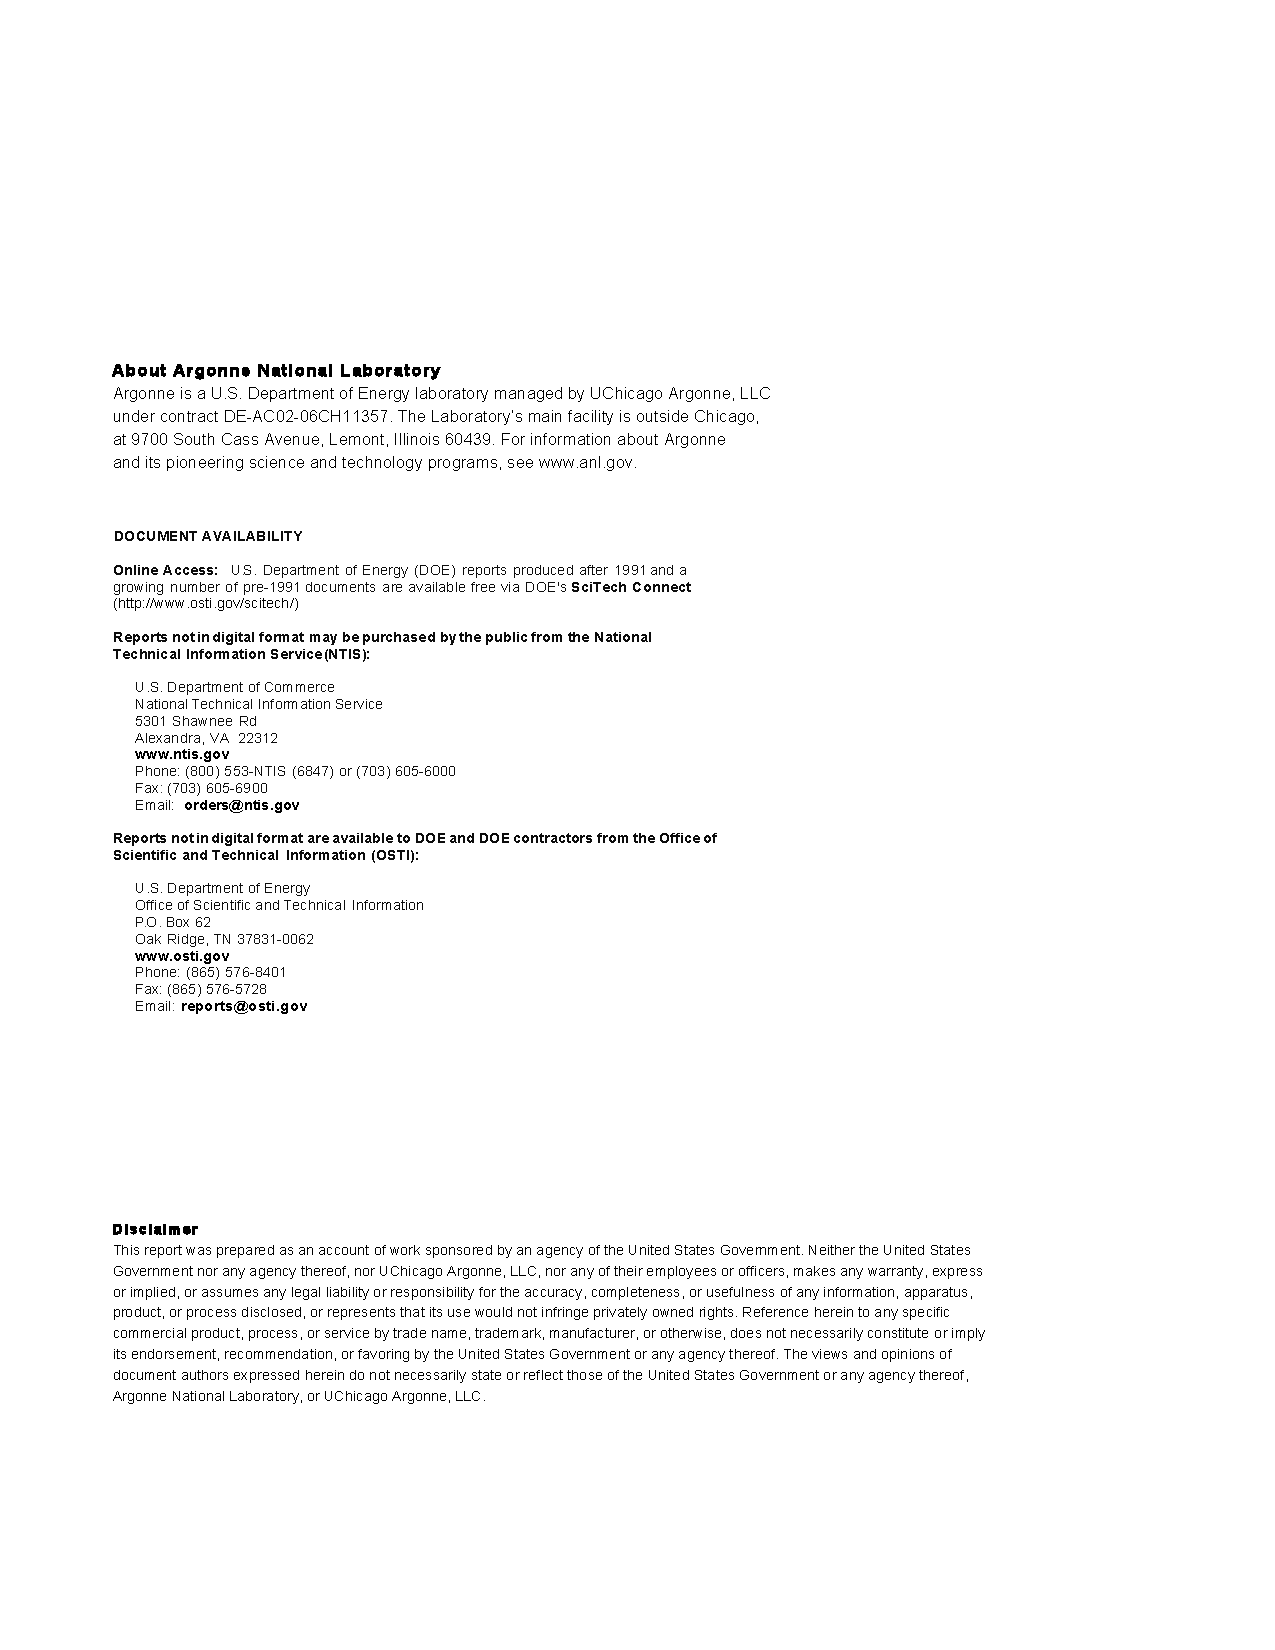
\includegraphics{ArgonneReportTemplatePage2}}
\restoregeometry
\newpage

%%%%%%%%%%%%%%%%%%%%%%%%%%%%%%%%%%%%%%%%%%%%%%%%%%%%%%%%%%%%%%%%%%%%%%%%%%%%%%%%%%%%

\pagestyle{empty}
\hfill {\large {\bf ANL-95/11 Rev 3.10}}

\vspace*{2in}
\noindent {\LARGE{\bf PETSc Users Manual}}
\vspace*{8pt}
\hrule
\vspace*{8pt}
\noindent {\Large{\it Revision 3.10}}

\vspace*{0.5in}
\noindent Prepared by \\
{\bf S. Balay\textsuperscript{1}, S. Abhyankar\textsuperscript{2}, M. Adams\textsuperscript{3}, J. Brown\textsuperscript{1}, P. Brune\textsuperscript{1}, K. Buschelman\textsuperscript{1},
L. Dalcin\textsuperscript{4}, A. Dener\textsuperscript{1}, V. Eijkhout\textsuperscript{6}, W. Gropp\textsuperscript{1}, D. Karpeyev\textsuperscript{1},
D. Kaushik\textsuperscript{1}, M. Knepley\textsuperscript{1}, D. May\textsuperscript{7}, L. Curfman McInnes\textsuperscript{1}, R. Mills\textsuperscript{1}, T. Munson\textsuperscript{1},
K. Rupp\textsuperscript{1}, P. Sanan\textsuperscript{8}, B. Smith\textsuperscript{1}, S. Zampini\textsuperscript{4}, H. Zhang\textsuperscript{5}, and H. Zhang\textsuperscript{1}}\\
\\
\textsuperscript{1}Mathematics and Computer Science Division, Argonne National Laboratory \\
\\
\textsuperscript{2}Energy Systems Division, Argonne National Laboratory \\
\\
\textsuperscript{3}Computational Research, Lawrence Berkeley National Laboratory \\
\\
\textsuperscript{4}Extreme Computing Research Center, King Abdullah University of Science and Technology\\
\\
\textsuperscript{5}Computer Science Department, Illinois Institute of Technology\\
\\
\textsuperscript{6}Texas Advanced Computing Center, University of Texas at Austin\\
\\
\textsuperscript{7}Department of Earth Sciences, University of Oxford\\
\\
\textsuperscript{8}Institute of Geophysics, ETH Zurich\\


\vspace*{30pt}
\noindent September 2018

\vspace*{20pt}
\noindent This work was supported by the Office of Advanced Scientific Computing Research, \\
Office of Science, U.S. Department of Energy, under Contract DE-AC02-06CH11357.


\cleardoublepage
%\pagestyle{plain}
\pagestyle{fancy}
\vspace{1in}
\date{\today}

% Abstract for users manual
\addcontentsline{toc}{chapter}{Abstract}
% Abstract for TAO Users Manual

\addcontentsline{toc}{chapter}{Preface}
\section*{Preface}

The Toolkit for Advanced Optimization (TAO) focuses on the development
of algorithms and software for the solution of large-scale optimization 
problems on high-performance architectures.  Areas of interest include 
unconstrained and bound-constrained optimization, nonlinear least squares 
problems, optimization problems with partial differential equation 
constraints, and variational inequalities and complementarity 
constraints.

The development of TAO was motivated by the scattered support for
parallel computations and the lack of reuse of external toolkits in
current optimization software.  Our aim is to produce high-quality 
optimization software for computing environments ranging from 
workstations and laptops to massively parallel high-performance 
architectures.  Our design decisions are strongly motivated by 
the challenges inherent in the use of large-scale distributed 
memory architectures and the reality of working with large, 
often poorly structured legacy codes for specific 
applications.

%%% Local Variables: 
%%% mode: latex
%%% TeX-master: "manual_tex"
%%% End: 



\cleardoublepage

\input{gettinginfo.tex}

\medskip \medskip

\cleardoublepage

% Acknowledgements for users manual
\input{acknowltmp.tex}

% Blank page makes double sided printout look bettter.

\cleardoublepage
\label{tableofcontents}
\tableofcontents

% --------------------------------------------------------------------
%                            PART 1
% --------------------------------------------------------------------
\cleardoublepage
\part{Introduction to PETSc}
\label{part_intro}
\cleardoublepage
\chapter{Getting Started}
\input{part1tmp.tex}

% --------------------------------------------------------------------
%                            PART 2
% --------------------------------------------------------------------
\cleardoublepage
\part{Programming with PETSc}
\label{part_usage}
\input{part2tmp.tex}


%------------------------------------------------------------------


\cleardoublepage
\bibliographystyle{plain}
\addtocounter{chapter}{1}
\addcontentsline{toc}{chapter}{Bibliography}
\label{sec:bib}
\bibliography{../petsc,../petscapp}

\pagestyle{empty}
\newgeometry{top=0mm, left=0mm, right=0mm, bottom=0mm}
\begin{figure*}[hbt]
\centerline{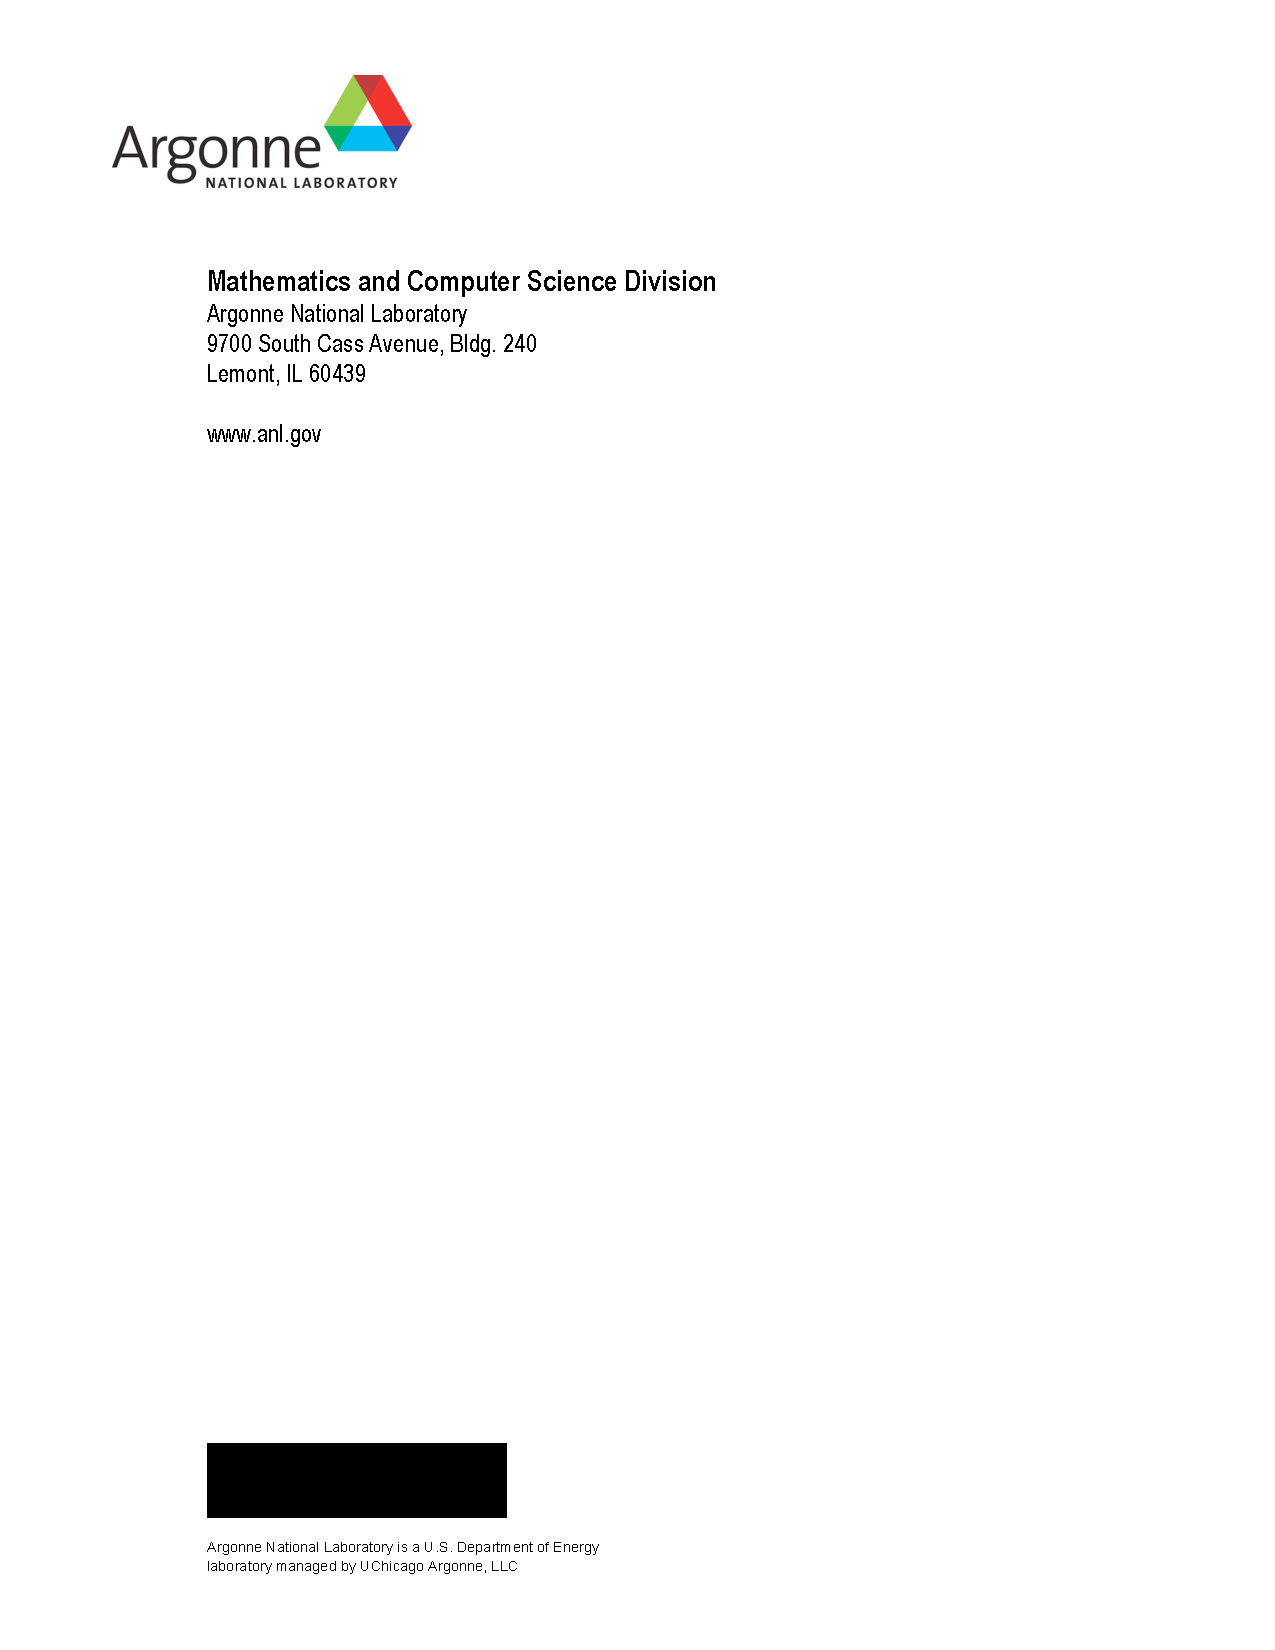
\includegraphics{ArgonneReportTemplateLastPage.pdf}}
\caption{}
\end{figure*}
\restoregeometry

\end{document}

%%% Local Variables:
%%% mode: latex
%%% TeX-master: t
%%% End:
